%\documentclass[9pt,handout]{beamer}
\documentclass{beamer}

\usepackage{amsmath, epsfig, subfigure, psfrag, amssymb, amsfonts, array, amsthm}
\usepackage{tikz}
	\usetikzlibrary{calc, shapes.geometric, positioning, shapes, decorations, arrows, patterns}
\usepackage{wasysym}
 \usetikzlibrary{decorations.markings}

\mode<presentation>

\usetheme{Pittsburgh}
\usecolortheme{beaver}
%\useoutertheme{split}

\setbeamertemplate{footline}{}%[split, frame number]
\setbeamertemplate{enumerate items}[default]
\setbeamertemplate{itemize items}[circle]

\setbeamersize{text margin left=6mm}
\setbeamersize{text margin right=6mm}
\setbeamersize{sidebar width right=0mm}
\setbeamersize{sidebar width left=0mm}
\setbeamertemplate{navigation symbols}{}

\newtheorem{comments}{Comments}
\newtheorem{question}{Question}
\newtheorem{goal}{Goal}
\newtheorem{remark}{Remark}
\newtheorem{proposition}{Proposition}
\newtheorem{conjecture}{Conjecture}

% \newcommand*\oldmacro{}
% \let\oldmacro\insertshorttitle
% \renewcommand*\insertshorttitle{
% \oldmacro\hfill
% \insertframenumber\,/\,\inserttotalframenumber}

\def\tsimkappa{\sim_{\kappa}}
\def\r{\vec{r}}
\newcommand{\w}{\overline{w}}
%\DeclareMathOperator{\Cyc}{Acyc}
\DeclareMathOperator{\FC}{FC}
\newcommand{\C}{\widetilde{C}}
\DeclareMathOperator{\Sym}{Sym}
\DeclareMathOperator{\supp}{supp}

%%%%%%%%%%%%%% Heap Code %%%%%%%%%%%%%%
\usetikzlibrary{patterns}

\newcommand\heapblock[4]{\fill[fill=#4, fill opacity=0.35, draw=#4, line width=1.1pt, rounded corners,shift={(\xxaxis:#1)},shift={(\yyaxis:#2)}] (-1,-1) rectangle (1,1);\node at (#1,#2) {\footnotesize $#3$};}

\newcommand\dheapblock[4]{\draw[dotted, draw=#4, line width=1.1pt, rounded corners,shift={(\xxaxis:#1)},shift={(\yyaxis:#2)}] (-1,-1) rectangle (1,1);\node at (#1,#2) {\footnotesize $#3$};}

\newcommand\sheapblock[4]{\draw[pattern= north west lines, pattern color=#4, draw=#4, line width=1.1pt, rounded corners,shift={(\xxaxis:#1)},shift={(\yyaxis:#2)}] (-1,-1) rectangle (1,1);\node at (#1,#2) {\footnotesize $#3$};}

\newcommand\xxaxis{0}
\newcommand\yyaxis{90}

\definecolor{orange}{RGB}{255,102,0}
\definecolor{ggreen}{RGB}{0,153,0}
\definecolor{darkblue}{RGB}{0,0,255}
\definecolor{purple}{RGB}{153,51,255}
\definecolor{turq}{RGB}{72,209,204}
\definecolor{gray}{RGB}{220,220,220}
\definecolor{orange2}{RGB}{255,100,0}
\definecolor{purple2}{RGB}{159,51,250}
\definecolor{rred}{rgb}{0.9, 0.17, 0.31}


%% ----------------------------------------------------------------------  

\begin{document}

\def\newblock{\hskip .11em plus .33em minus .07em}

\title[A Study of T-Avoiding Elements in Coxeter Groups]
{\textbf{A Study of T-Avoiding Elements in Coxeter Groups}}
\author[T.M.~Laird]{Taryn Laird}
\institute[NAU]{Northern Arizona University\\
Department of Mathematics and Statistics}

\vspace{1em}

\date[NAU]{\textbf{NAU Thesis Defense}\\
April 29, 2016}

\frame{\titlepage}

%% ----------------------------------------------------------------------



\begin{frame}{\textbf{Coxeter Systems}}

\begin{definition}
A \alert{Coxeter system} consists of a group $W$ (called a \alert{Coxeter group}) generated by a set $S$ of involutions with presentation
\[ W=\langle S \mid s^2=e, (st)^{m(s,t)}=e \rangle \]

where $m(s,t) \geq 2$ for all $s \neq t$.
\end{definition}

\pause

\begin{block}{Comment}
Since $s$ and $t$ are involutions, the relation $(st)^{m(s,t)}=e$ can be 
rewritten as

\begin{center}
\begin{tabular}{ll}
$\left.\begin{array}{lcc}m(s,t)=2 & \implies &\ \ \, st=ts\ \   \end
{array}\right\}$&  \alert{commutations}\\
\\\pause
$\left.\begin{array}{lcc}m(s,t)=3 & \implies & sts=tst \\
& & \\
m(s,t)=4 & \implies & stst=tsts \\
 & \vdots &  \end{array}\right\}$ &\alert{braid relations}
\end{tabular}
\end{center}
\end{block}
\end{frame}

%% ----------------------------------------------------------------------

\begin{frame}{\textbf{Coxeter Graphs}}

\begin{definition}
We can encode $(W,S)$ with a unique \alert{Coxeter graph} $\Gamma$ having: 

\begin{itemize}
\item vertex set $S$;

\item edges $\{s,t\}$ labeled $m(s,t)$ whenever $m(s,t)\geq 3;$



\end{itemize}

\vspace{-1em}

\end{definition}

\pause

\begin{block}{Comments}
\begin{itemize}

\item if $m(s,t)=3$, we omit label.

\item If $s$ and $t$ are not connected in $\Gamma$, then $s$ and $t$ 
commute.

\item Given $\Gamma$, we can uniquely reconstruct the corresponding $(W,S)
$. 

\end{itemize}

\end{block}

\end{frame}

%% ----------------------------------------------------------------------

\begin{frame}{\textbf{Coxeter groups of type $A$}}

Coxeter groups of type $A_{n}$ ($n\geq 1$) are defined by:
\begin{figure}
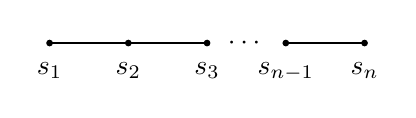
\begin{tikzpicture}
\draw[fill=black] \foreach \x in {1,2,3,4,5} {(\x,10) circle (1pt)};
\draw \foreach \x in {1,2,3} {(\x,10) node[label=below:$s_{\x}$]{}};
\draw {(4,10) node[label=below:$s_{n-1}$]{}};
\draw {(5,10) node[label=below:$s_{n}$]{}};
\draw {(3.5,10) node[]{$\cdots$}};
\draw[-] (1,10) -- (3,10);
\draw[-] (4,10) -- (5,10);
\end{tikzpicture}
\end{figure}

\pause
 
Then $W(A_{n})$ is generated by $\{s_{1}, s_{2}, \cdots, 
s_{n}\}$ and is subject to defining relations
\begin{enumerate}
\item $s_{i}^{2}=1$ for all $i$,
\item $s_{i}s_{j}=s_{j}s_{i}$ if $|i-j|>1$,
\item $s_{i}s_{j}s_{i}=s_{j}s_{i}s_{j}$ if $|i-j|=1$.
\end{enumerate}
\pause 
$W(A_{n})$ is isomorphic to the symmetric group, $Sym_{n+1}$, under 
the correspondence 
\[
s_{i}\mapsto (i,\ i+1),
\]
where $(i,\ i+1)$ is the adjacent transposition exchanging $i$ and $i+1$.

\end{frame}

%% ----------------------------------------------------------------------

\begin{frame}{\textbf{Coxeter groups of type $B$}}

Coxeter groups of type $B_{n}$ ($n\geq 2$) are defined by: 
\begin{figure}
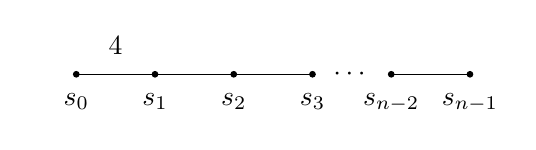
\begin{tikzpicture}[scale=1.0]%B_{n}
\draw [fill=black] \foreach \x in {1,2,...,6} {(\x,8.5) circle (1pt)};
%\draw [fill=white] (1,10) circle(2pt);
\draw {(.5,8.5) node{}
(1.5,8.5) node[label=above:$4$]{}
(6,8.5) node[label=above:\textcolor{white}{$4$}]{}
(4.5,8.5) node{$\cdots$}
(1,8.5) node[label=below:$s_0$]{}
(2,8.5) node[label=below:$s_1$]{}
(3,8.5) node[label=below:$s_2$]{}
(4,8.5) node[label=below:$s_3$]{}
(5,8.5) node[label=below:$s_{n-2}$]{}
(6,8.5) node[label=below:$s_{n-1}$]{}
[-] (1,8.5) -- (4,8.5)
[-] (5,8.5) -- (6,8.5)
(2,8.5) node{}}; 
\end{tikzpicture}
\end{figure}

\pause

Then $W(B_{n})$ is generated by $\{s_{1}, s_{2}, 
\cdots, s_{n-1}\}$ and is subject to defining relations 
\begin{enumerate}
\item $s_{i}^{2}=1$ for all $i$, 
\item $s_{i}s_{j}=s_{j}s_{i}$ if $|i-j|>1$, 
\item $s_{i}s_{j}s_{i}=s_{j}s_{i}s_{j}$ if $|i-j|=1$ and $1<i,j\leq n$, 
\item $s_{0}s_{1}s_{0}s_{1}=s_{1}s_{0}s_{1}s_{0}$.
\end{enumerate}
\pause $W(B_{n})$ is a finite group of order $n!2^{n}$ (wreath product of 
$\mathbb{Z}_{2}$ and the symmetric group).

\end{frame}

%% ----------------------------------------------------------------------


\begin{frame}{\textbf{Coxeter groups of type affine $C$}}

Coxeter groups of type $\C_{n}$ ($n \geq 2$) are defined by:
\begin{figure}
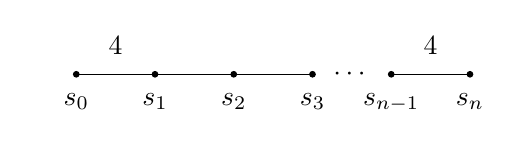
\begin{tikzpicture}[scale=1.0]
\draw[fill=black] \foreach \x in {1,2,...,6} {(\x,5) circle (1pt)};%\widetild{C}_{n}
%\fill[white] (1,6) circle (2pt);
\draw {(.5,5) node{}
(4.5,5) node{$\cdots$}
(5.5,5) node[label=above:$4$]{}
(1.5,5) node[label=above:$4$]{}
(1,5) node[label=below:$s_0$]{}
(2,5) node[label=below:$s_1$]{}
(3,5) node[label=below:$s_2$]{}
(4,5) node[label=below:$s_3$]{}
(5,5) node[label=below:$s_{n-1}$]{}
(6,5) node[label=below:$s_{n}$]{}
[-] (1,5) -- (4,5)
[-] (5,5) -- (6,5)
(2,5) node{}};
\end{tikzpicture}
\end{figure}

\pause 
Here, we see that $W(\C_{n})$ is generated by $\{s_{0}, 
\cdots, s_{n}\}$ and is subject to defining relations
\begin{enumerate}
\item $s_{i}^{2}=1$ for all $i$,
\item $s_{i}s_{j}=s_{j}s_{i}$ if $|i-j|>1$,
\item $s_{i}s_{j}s_{i}=s_{j}s_{i}s_{j}$ if $|i-j|=1$ and $1< i,j < n+1$, 
\item $s_{i}s_{j}s_{i}s_{j}=s_{j}s_{i}s_{j}s_{i}$ if $\{i,j\}=\{0,1\}$ or 
$\{n-1,n\}$.
\end{enumerate}
\pause 
\bigskip
$W(\C_{n})$ is an infinite group.

\pause

\begin{block}{Comment}
We can obtain $W(A_{n})$ and $W(B_{n})$ from $W(\C_{n})$ by removing the 
appropriate generators and corresponding relations.  In fact, 
we can obtain $W(B_{n})$ in two ways.
\end{block}

\end{frame}

%% ----------------------------------------------------------------------

\begin{frame}{\textbf{Reduced expressions}}

\begin{block}{Definition}
A word $s_{x_1}s_{x_2}\cdots s_{x_m}\in S^{*}$ is called an \alert
{expression} for $w\in W$ if it is equal to $w$ when considered as 
a group element.

\vspace{1em}
\pause

If $m$ is minimal, it is a \alert{reduced expression}, and the \alert
{length} of $w$ is $\ell(w):=m$.

\vspace{1em}
\pause

Given $w \in W$, if we wish to emphasize a fixed, possibly reduced, 
expression for $w$, we represent it as
\[
\w=s_{x_1}s_{x_2}\cdots s_{x_m}.
\]
\end{block}

\end{frame}

%% -------------------------------------------------------------------

\begin{frame}{\textbf{Matsumoto's Theorem and Support}}
\begin{block}{Theorem (Matsumoto)}
Any two reduced expressions for $w\in W$ differ by a sequence of commutations and braid moves.
\end{block}	

\pause

\begin{definition}
	We define $\supp(w)$ to be the set of generators appearing in any reduced expression for $w$. This is well defined by Matsumoto's theorem.
\end{definition}

\pause

\begin{example}
Let $\w=s_2s_1s_2s_3s_1$ be a fixed expression for $w \in W(A_3)$. We see that
\[\alert{s_2s_1s_2}s_3s_1 \pause =s_1s_2s_1\alert{s_3s_1} \pause =s_1s_2\alert{s_1s_1}s_3\pause=s_1s_2s_3\]	
This implies that $\w$ was not reduced. However, it turns out that $s_1s_2s_3$ is a reduced expression for $w$. Then $\supp(w)=\{s_1s_2s_3\}$ and $\ell(w)=3$.
\end{example}

\end{frame}


%% -------------------------------------------------------------------
\begin{frame}{\textbf{Fully Commutative Elements}}
\begin{definition}
Let $(W,S)$ be a Coxeter system of type $\Gamma$. We say that $w \in W(\Gamma)$ is \alert{fully commutative} (\alert{FC}) if any two reduced expressions for $w$ can be transformed into each other via iterated commutations. The set of FC elements is denoted $\FC(\Gamma)$.	
\end{definition}

\begin{block}{Theorem (Stembridge)}
$w \in \FC(\Gamma)$ if and only if no reduced expression for $w$ contains a braid.
\end{block}

\begin{block}{Comment}
	It follows from Stembridge that $W(\C_n)$ contains an infinite number of FC elements, while $W(A_n)$ and $W(B_n)$ do not. 
\end{block}

\end{frame}

%% -------------------------------------------------------------------

\begin{frame}{Fully Commutative Elements}
\begin{block}{Comment}
	The elements of $\FC(\C_n)$ are precisely those whose reduced expressions avoid the consecutive subwords $s_is_js_i$ for $m(s_i,s_j)=3$, $s_0s_1s_0s_1$, and $s_{n-1}s_ns_{n-1}s_n$.
\end{block}

\pause

\begin{block}{Example}
	Let $\w=s_0s_2s_4s_3s_2s_1$ be a reduced expression for $w \in W(\C_4)$. We see that
	\[s_0\alert{s_2s_4}s_3s_2s_1=s_0s_4\alert{s_2s_3s_2}s_1.\]
	Since $w$ has one of the forbidden consecutive subwords, $w$ is \alert{not} FC.
\end{block}
		
\end{frame}

%% -------------------------------------------------------------------

\begin{frame}{Heaps}
We introduce \alert{heaps} through an example.

\pause

\begin{block}{Example}
Let $\w=s_4s_5s_1s_0s_2s_4s_1$ be a reduced expression for $w \in W(B_6)$.
\begin{columns}
\begin{column}{0.4\textwidth}
\begin{figure}\centering
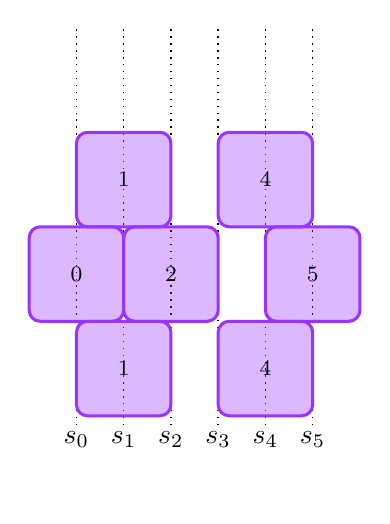
\begin{tikzpicture}[scale=0.6]
\node at (0.5,-2.5) {$ $};
\node at (0,-1.5) {$s_0$};
\node at (1,-1.5) {$s_1$};
\node at (2,-1.5) {$s_2$};
\node at (3,-1.5) {$s_3$};
\node at (4,-1.5) {$s_4$};
\node at (5,-1.5) {$s_5$};
\draw[dotted, line width=0.5pt] (1,-1.2) -- (1,7.2);
\draw[dotted, line width=0.5pt] (2,-1.2)   -- (2,7.2);
\draw[dotted, line width=0.5pt] (3,-1.2) -- (3,7.2);
\draw[dotted, line width=0.5pt] (4,-1.2)   -- (4,7.2);
\draw[dotted, line width=0.5pt] (5,-1.2) -- (5,7.2);
\draw[dotted, line width=0.5pt] (0,-1.2) -- (0, 7.2); \pause

\heapblock{1}{0}{1}{purple}\pause
\heapblock{0}{2}{0}{purple}\pause
\heapblock{2}{2}{2}{purple}\pause
\heapblock{4}{0}{4}{purple}\pause
\heapblock{1}{4}{1}{purple}\pause
\heapblock{5}{2}{5}{purple}\pause
\heapblock{4}{4}{4}{purple}

\end{tikzpicture}	
\end{figure}
\end{column}
\pause
\begin{column}{0.4\textwidth}
\begin{figure}\centering
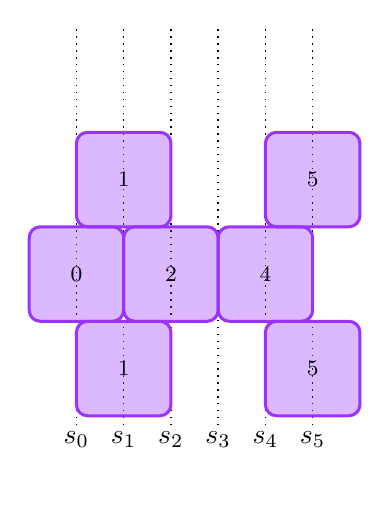
\begin{tikzpicture}[scale=0.6]
	\node at (0.5,-2.5) {$ $};
\node at (0,-1.5) {$s_0$};
\node at (1,-1.5) {$s_1$};
\node at (2,-1.5) {$s_2$};
\node at (3,-1.5) {$s_3$};
\node at (4,-1.5) {$s_4$};
\node at (5,-1.5) {$s_5$};
\draw[dotted, line width=0.5pt] (1,-1.2) -- (1,7.2);
\draw[dotted, line width=0.5pt] (2,-1.2)   -- (2,7.2);
\draw[dotted, line width=0.5pt] (3,-1.2) -- (3,7.2);
\draw[dotted, line width=0.5pt] (4,-1.2)   -- (4,7.2);
\draw[dotted, line width=0.5pt] (5,-1.2) -- (5,7.2);
\draw[dotted, line width=0.5pt] (0,-1.2) -- (0, 7.2); 

\heapblock{1}{0}{1}{purple}
\heapblock{0}{2}{0}{purple}
\heapblock{2}{2}{2}{purple}
\heapblock{5}{0}{5}{purple}
\heapblock{1}{4}{1}{purple}
\heapblock{4}{2}{4}{purple}
\heapblock{5}{4}{5}{purple}
\end{tikzpicture}
\end{figure}	
\end{column}
\end{columns}
\end{block}
	
\end{frame}

%% -------------------------------------------------------------------


\end{document}